% ---------
%  Compile with "pdflatex hw0".
% --------
%!TEX TS-program = pdflatex
%!TEX encoding = UTF-8 Unicode

\documentclass[11pt]{article}
\usepackage{amsmath}
\usepackage{amssymb}
\usepackage{jeffe,handout,graphicx}
\usepackage[utf8]{inputenc}		% Allow some non-ASCII Unicode in source

% =========================================================
%   Define common stuff for solution headers
% =========================================================
\pagenumbering{arabic}
\Class{ECE 498 ICC}
\Semester{Spring 2020}
\Authors{1}
\AuthorOne{Jin Yucheng}{yucheng9}
%\AuthorTwo{Friday Caliban}{fcaliban}
%\AuthorThree{Duncan Quagmire}{dquagmir}
%\Section{}

% =========================================================
\begin{document}

% ---------------------------------------------------------


\HomeworkHeader{2}{1}	% homework number, problem number

\begin{solution}
(1) One advantage is that using IP-based hardware design, we can make the computation process faster (by parallel computation, for example). One disadvantage is that using IP-based hardware design, we may sacrifice some flexibility. 
\item
(2) For (a), we need $128$ compute engine IPs: $\frac{2n}{0.25n} \times \frac{4n}{0.25n} = 128$.
\item For (b), we need $32$ compute engine IPs: $\frac{2n}{0.5n} \times \frac{4n}{0.5n} = 32$.
\item
(3) Since $k$ IPs are instantiated, and each IP is of version (b) from part (2), we have,
\begin{itemize}
\item Area = $k \cdot A$ + $32 \times \frac{1}{4} A$ = $(k + 8) A$
\item Latency = $(T + \frac{k^2}{32}T) \cdot \frac{32}{k}$ = $(\frac{32}{k} + k)T$
\item Area $\times$ Latency = $(k + 8) A \cdot (\frac{32}{k} + k)T$ = $(k^2+8k+32+\frac{256}{k})AT$
\end{itemize}
The objective function, $f = (k^2+8k+32+\frac{256}{k})$ is minimized at $k = 4$. Because $\frac{df}{dk} = 2k + 8 - \frac{256}{k^2}$ equals $0$ at $k = 4$, and $\frac{df}{dk} > 0$ for $k > 4$, $f$ is monotonously increasing; $\frac{df}{dk} < 0$ for $k < 4$, $f$ is monotonously decreasing, therefore, $f$ is minimized at $k = 4$.
\item In conclusion, $4$ IPs should be instantiated to minimize the product of total latency and total area.
\begin{center}
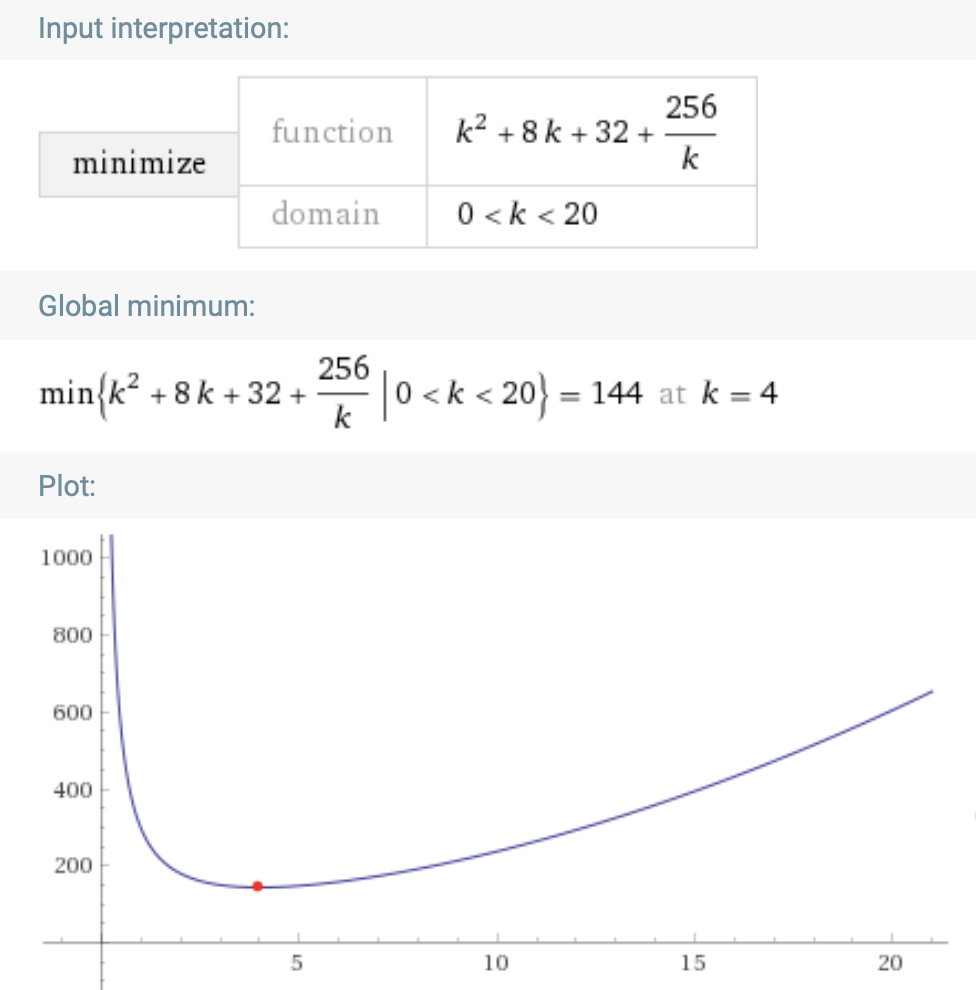
\includegraphics[width=10cm]{1.png}
\end{center}
\end{solution}
% ---------------------------------------------------------
\HomeworkHeader{2}{2}	% homework number, problem number
\setcounter{page}{2}
\begin{solution}
(1) \item \qquad \underline{Conv\_Layer\_One(img$[3][28][28]$, conv\_weight$[3][3][5][5]$):}
\item \qquad $\text{  } 1 \text{   }:$\textbf{ for} $i$ $\leftarrow 1$ to $3$:
\item \qquad $\text{  } 2 \text{   }:$\qquad  \textbf{ for} $j \leftarrow 1$ to $24$: 
\item \qquad $\text{  } 3 \text{   }:$\qquad  \qquad  \textbf{ for} $k \leftarrow 1$ to $24$: 
\item \qquad $\text{  } 4 \text{   }:$\qquad  \qquad \qquad conv$1[i][j][k]=0$ 
\item \qquad $\text{  } 5 \text{   }:$\qquad  \qquad \qquad \qquad  \textbf{ for} $x \leftarrow 1$ to $3$: 
\item \qquad $\text{  } 6 \text{   }:$\qquad  \qquad \qquad \qquad \qquad \textbf{ for} $y \leftarrow 1$ to $5$: 
\item \qquad $\text{  } 7 \text{   }:$\qquad  \qquad \qquad \qquad \qquad \qquad \textbf{ for} $z \leftarrow 1$ to $5$: 
\item \qquad $\text{  } 8 \text{   }:$\qquad  \qquad \qquad \qquad \qquad \qquad \qquad conv$1[i][j][k]$ += img$[x][y+j][z+k]$ *
\item \qquad $\text{  } 9\text{   }:$\qquad  \qquad \qquad \qquad \qquad \qquad \qquad \qquad \qquad \qquad \qquad conv\_weight$[i][x][y][z]$
\item \qquad $\text{  } 10:$\qquad  \qquad \qquad \qquad \qquad \qquad \textbf{end} 
\item \qquad $\text{  } 11:$\qquad  \qquad \qquad \qquad \qquad  \textbf{end} 
\item \qquad $\text{  } 12:$\qquad  \qquad \qquad \qquad \textbf{end} 
\item \qquad $\text{  } 13:$\qquad  \qquad  \textbf{end} 
\item \qquad $\text{  } 14:$\qquad    \textbf{end} 
\item \qquad $\text{  } 15:$  \textbf{end} 
\item \qquad $\text{  } 16:$ \# ReLu as activation function
\item \qquad $\text{  } 17:$\textbf{ for} $i$ $\leftarrow 1$ to $3$:
\item \qquad $\text{  } 18:$\qquad  \textbf{ for} $j \leftarrow 1$ to $24$: 
\item \qquad $\text{  } 19:$\qquad  \qquad  \textbf{ for} $k \leftarrow 1$ to $24$: 
\item \qquad $\text{  } 20:$\qquad  \qquad \qquad  \textbf{ if} conv$1[i][j][k] < 0$: conv$1[i][j][k] = 0$ 
\item \qquad $\text{  } 21:$\qquad \qquad \textbf{ end}
\item \qquad $\text{  } 22:$ \qquad  \textbf{ end}
\item \qquad $\text{  } 23:$   \textbf{ end}
\item Output: conv$1[3][24][24]$
\item
 \item \qquad \underline{Fully\_Connected\_Layer\_One(pool$2[3][6][6]$, fc\_weight$[100][108]$):}
\item \qquad $\text{  } 1 \text{   }:$ flatten = zeros$(108)$
\item \qquad $\text{  } 2 \text{   }:$\textbf{ for} $i$ $\leftarrow 1$ to $3$:
\item \qquad $\text{  } 3 \text{   }:$\qquad  \textbf{ for} $j \leftarrow 1$ to $6$: 
\item \qquad $\text{  } 4 \text{   }:$\qquad  \qquad  \textbf{ for} $k \leftarrow 1$ to $6$: 
\item \qquad $\text{  } 5 \text{   }:$\qquad  \qquad \qquad flatten$[6 * 6 * i + 6 * j + k]$ = pool$2[i][j][k]$ 
\item \qquad $\text{  } 6 \text{   }:$\qquad  \qquad \textbf{ end}
\item \qquad $\text{  } 7 \text{   }:$ \qquad \textbf{ end}
\item \qquad $\text{  } 8 \text{   }:$\textbf{ end}
\item \qquad $\text{  } 9 \text{   }:$\textbf{ for} $i$ $\leftarrow 1$ to $100$:
\item \qquad $\text{  } 10:$ \qquad fc$1[i]$ = $0$ 
\item \qquad $\text{  } 11:$\qquad  \textbf{ for} $j$ $\leftarrow 1$ to $108$:
\item \qquad $\text{  } 12:$\qquad  \qquad fc$[i]$ += fc\_weight$[i][j]$ * flatten$[j]$
\item \qquad $\text{  } 13:$\qquad  \textbf{ end} 
\item \qquad $\text{  } 14:$ \textbf{end} 
\item \qquad $\text{  } 15:$ \# ReLu as activation function
\item \qquad $\text{  } 16:$\textbf{for} $i$ $\leftarrow 1$ to $100$:
\item \qquad $\text{  } 17:$\qquad \textbf{if} fc$1[i]$ < $0$: fc$1[i]$ = $0$
\item \qquad $\text{  } 18:$\qquad  \textbf{end}
\item \qquad $\text{  } 19:$\textbf{end}
\item Output: fc$1[100]$
\item (2) \textbf{\# of floating-point operations in a convolutional layer} = \# of input channels $\times$ \# of output channels $\times$ output width $\times$ output height $\times$ filter size $\times 2$ (in this case \# of floating-point additions = \# of floating-point multiplications)
\item \textbf{\# of floating-point operations in a fully-connected layer} = input size $\times$ output size $\times 2$ (in this case \# of floating-point additions = \# of floating-point multiplications)
\begin{itemize}
\item For convolutional layers: $Flop_{conv}$ = $3 \times 24 \times 24 \times 3 \times 5 \times 5 \times 2$ + $3 \times 12 \times 12 \times 3 \times 3 \times 3 \times 2 = 282,528$
\item For fully-connected layers: $Flop_{fc}$ = $108 \times 100 \times 2 + 100 \times 50 \times 2 +  50 \times 10 \times 2 = 32,600$
\item Total \# of floating-point operations = $282,528 + 32,600 = 315,128$
\item \% of floating-point operations in convolutional layers: $\frac{282,528}{315,128} \times 100\%$ = $89.655\%$
\item \% of floating-point operations in fully-connected layers: $\frac{32,600}{315,128} \times 100\%$ = $10.345\%$
\end{itemize}
Therefore, convolutional layers take the majority of floating-point operations. 
\item (3) Assume each parameter takes 32-bit. Assume there is no bias in any layers.
\item \textbf{\# of parameters in a convolutional layer} =  \# of input channels $\times$ \# of output channels $\times$ filter size
\item \textbf{\# of parameters in a fully-connected layer} =  input size $\times$ output size
\begin{itemize}
\item For convolutional layers: $Para_{conv}$ = $3 \times 3 \times 5 \times 5 \times 4 \times \frac{1}{1024^2}$ + $3 \times 3 \times 3 \times 3 \times 4 \times \frac{1}{1024^2} = 0.0011673$ [MB]
\item For fully-connected layers: $Para_{fc}$ = $108 \times 100 \times 4 \times \frac{1}{1024^2} + 100 \times 50 \times 4 \times \frac{1}{1024^2} +  50 \times 10 \times 4 \times \frac{1}{1024^2} = 0.0621796$ [MB]
\item Total size of parameters = $0.0011673 + 0.0621796 = 0.0633469$ [MB]
\item \% of parameters in convolutional layers: $\frac{0.0011673}{0.0633469} \times 100\%$ = $1.84\%$
\item \% of parameters in fully-connected layers: $\frac{0.0621796}{0.0633469} \times 100\%$ = $98.16\%$
\end{itemize}
Therefore, fully-connected layers take the majority of parameters.
\item(4) 
\begin{itemize}
\item For convolutional layers: $Ratio$ = $\frac{282,528}{0.0011673} \times 100\% = 242,035,466$
\item For fully-connected layers: $Ratio$ = $\frac{32,600}{0.0621796} \times 100\% = 524,288$
\end{itemize}
Because convolutional layers have a much larger computation-to-memory ratio, so each parameter in convolutional layers involves in more computations.
\item (5) Convolutional layers take the majority of floating-point operations in terms of computation, fully-connected layers take the majority of parameters in terms of memory, also, because convolutional layers have a much larger computation-to-memory ratio, so each parameter in convolutional layers performs more computations than each parameter in fully-connected layers. In conclusion, for a convolutional layer and a fully-connected layer with similar input sizes and output sizes, the convolutional layer has smaller number of parameters, but each parameter performs more computations, which results in higher amount of computation.
\end{solution}
% ---------------------------------------------------------
\HomeworkHeader{2}{3}	% homework number, problem number
\setcounter{page}{5}
\begin{solution}
(1) We have,
\begin{center}
$\mu_{X} = \frac{1}{m} \Sigma_{i=1}^m X[i]$
\item
$\sigma_{X}^2 = \frac{1}{m} \Sigma_{i=1}^m (X[i]-\mu_X)^2$
\item
$Y[i] = \gamma \frac{X[i] - \mu_X}{\sqrt{\sigma_X^2+\epsilon}}+\beta$
\end{center}
where $X[m] = \{x_{1...m}\}$ is a mini-batch, $\beta, \gamma$ are parameters to be learned, $\epsilon$ is a sufficiently small number to prevent division by zero, and $Y[m] = \{y_{1...m}\}$ is the output after applying batch normalization.
\item Batch normalization is a training technique that is used to normalize the output of the previous layer for each batch. After batch normalization, the mean of output will be close to $0$, and the standard deviation will be close to $1$.
\item(2) The Keras API is as follows (see https://keras.io/layers/normalization/), 
 \begin{center}
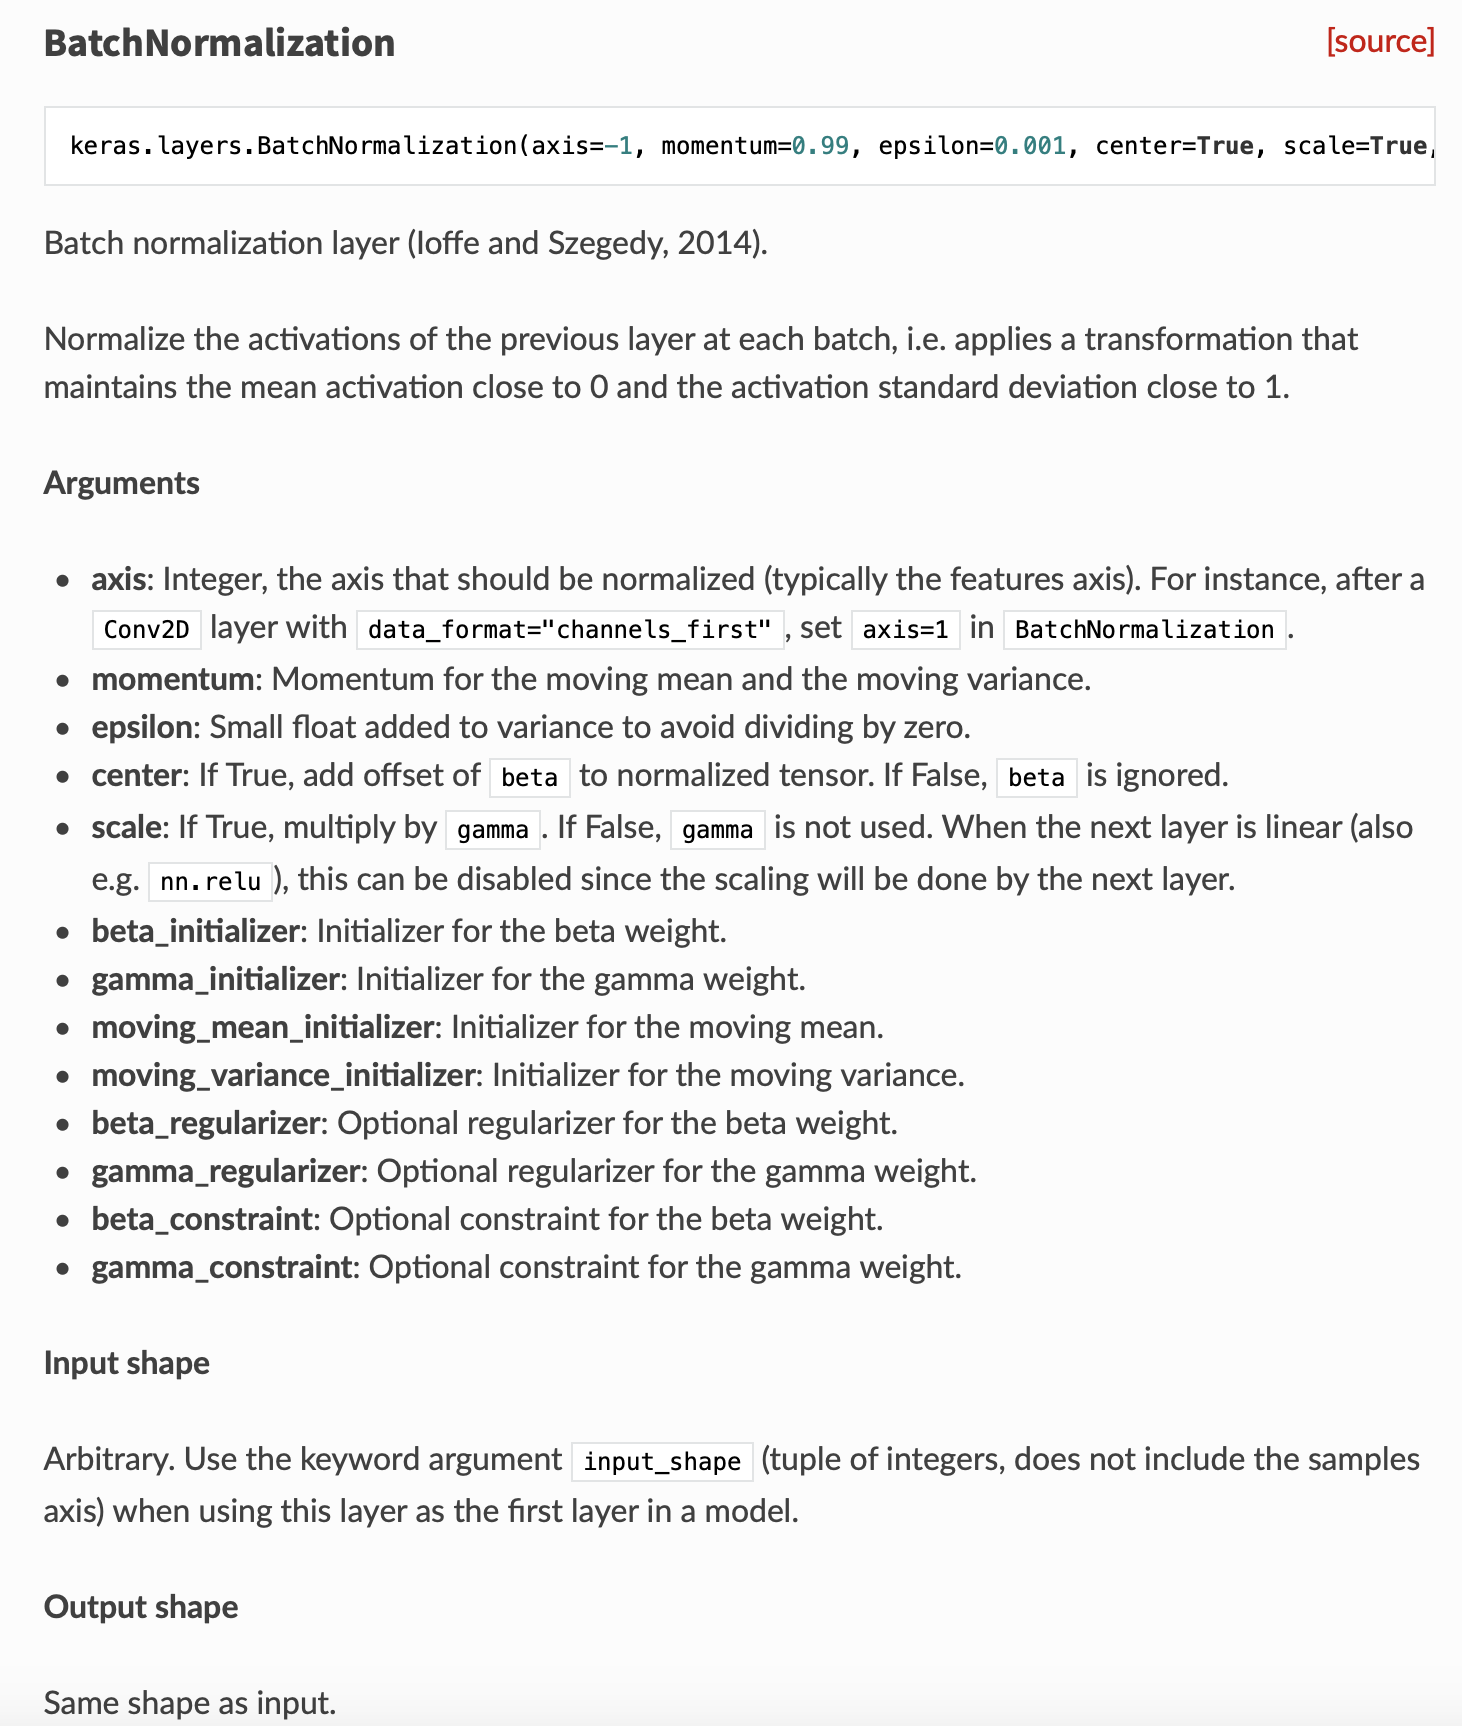
\includegraphics[width=11.5cm]{batch.png}
\end{center}
Therefore, my CNN is (batch normalization at line 8),
\begin{center}
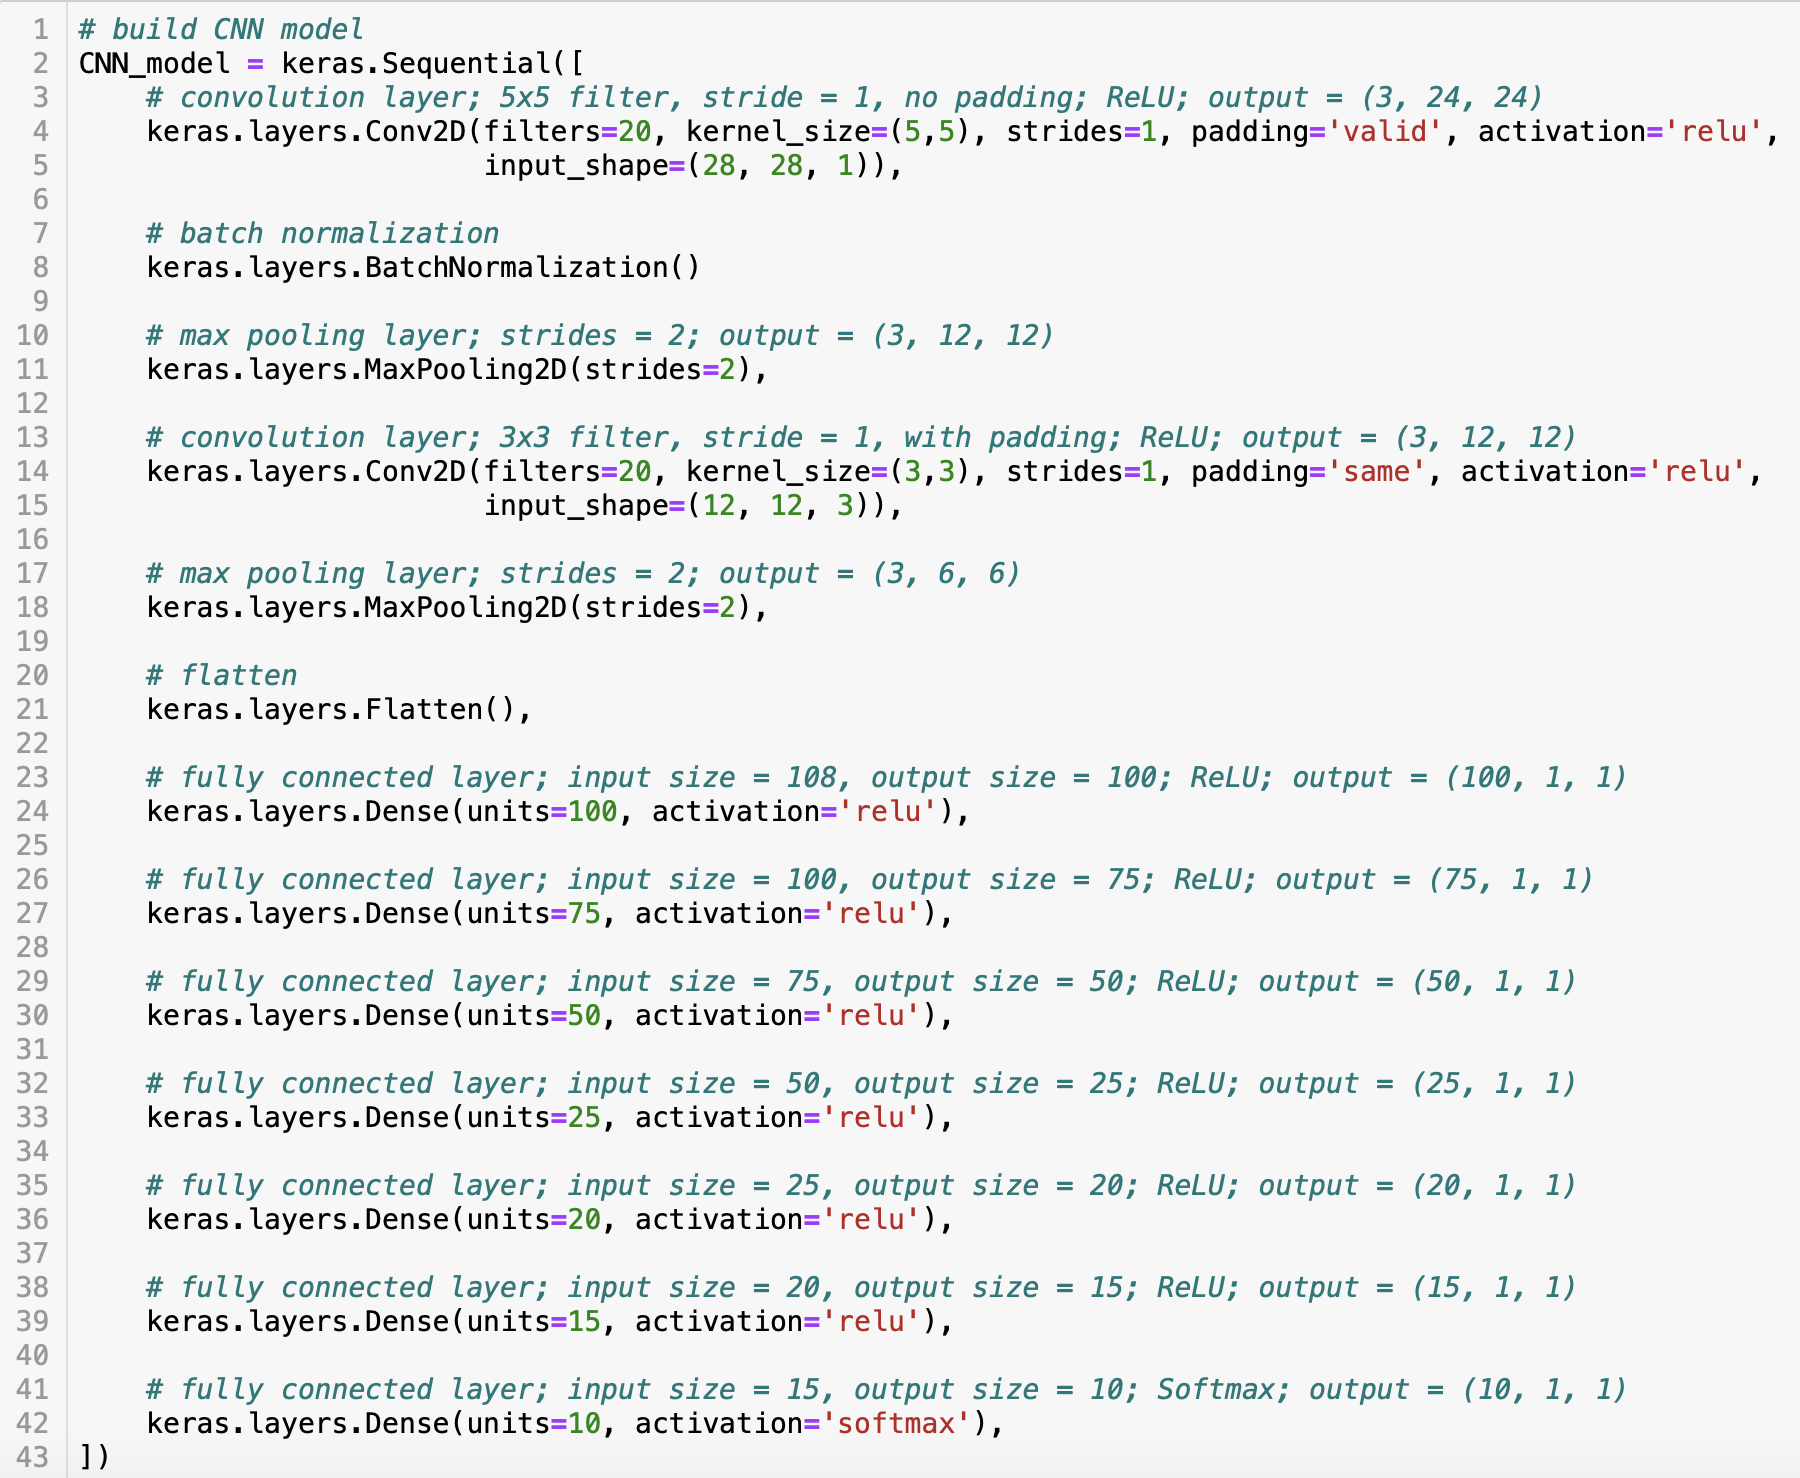
\includegraphics[width=15cm]{code.png}
\end{center}
\item(3) Yes, we can merge batch normalization into the convolutional layer. What we should do is just to modify weights and biases according to the following pseudocode,
 \item \qquad \underline{Batch\_Normalization\_Conv\_Layer(image$[C_{i}][H_{i}][W_{i}]$, conv\_weight$[C_o][C_i][H_o][W_o]$,} 
\item \qquad \underline{conv\_bias$[C_o]$, $\mu_X, \sigma_X^2, \beta, \gamma, \epsilon$)}:
\item \qquad $\text{  } 1 \text{   }:$\textbf{ for} $i$ $\leftarrow 1$ to $C_o$:
\item \qquad $\text{  } 2 \text{   }:$\qquad \textbf{ for} $j$ $\leftarrow 1$ to $C_i$:
\item \qquad $\text{  } 3 \text{   }:$\qquad \qquad  \textbf{ for} $k \leftarrow 1$ to $H_o$: 
\item \qquad $\text{  } 4 \text{   }:$\qquad  \qquad \qquad  \textbf{ for} $q \leftarrow 1$ to $W_o$: 
\item \qquad $\text{  } 5 \text{   }:$\qquad  \qquad \qquad \qquad conv\_weight[i][j][k][q] *= $\frac{\gamma[m]}{\sqrt{\sigma_X^2[m]+\epsilon}}$
\item \qquad $\text{  } 6 \text{   }:$\qquad \qquad \qquad \textbf{ end}
\item \qquad $\text{  } 7 \text{   }:$ \qquad \qquad \textbf{ end}
\item \qquad $\text{  } 8 \text{   }:$ \qquad \textbf{ end}
\item \qquad $\text{  } 9 \text{   }:$\textbf{ end}
\item \qquad $\text{  } 10:$\textbf{ for} $i$ $\leftarrow 1$ to $C_o$:
\item \qquad $\text{  } 11:$\qquad conv\_bias[i] = conv\_bias[i] * $\frac{\gamma[m]}{\sqrt{\sigma_X^2[m]+\epsilon}}$ + $\beta[m]$ - $\frac{\gamma[m]*\mu_X[m]}{\sqrt{\sigma_X^2[m]+\epsilon}}$
\item \qquad $\text{  } 12:$\textbf{ end}
\item \qquad $\text{  } 13:$\textbf{ for} $i$ $\leftarrow 1$ to $C_o$:
\item \qquad $\text{  } 14:$\qquad \textbf{ for} $j$ $\leftarrow 1$ to $H_i - H_o +1$:
\item \qquad $\text{  } 15:$\qquad\qquad \textbf{ for} $k$ $\leftarrow 1$ to $W_i - W_o + 1$:
\item \qquad $\text{  } 16:$\qquad\qquad\qquad\textbf{ for} $x$ $\leftarrow 1$ to $C_i$:
\item \qquad $\text{  } 17:$\qquad\qquad\qquad\qquad\textbf{ for} $y$ $\leftarrow 1$ to $H_o$:
\item \qquad $\text{  } 18:$\qquad\qquad\qquad\qquad\qquad\textbf{ for} $z$ $\leftarrow 1$ to $W_o$:
\item \qquad $\text{  } 19:$\qquad\qquad\qquad\qquad\qquad \qquad conv$1$[i][j][k] += image[x][j+y][k+z] * conv\_weight[i][x][y][z]
\item \qquad $\text{  } 20:$\qquad\qquad\qquad\qquad\qquad\textbf{ end}
\item \qquad $\text{  } 21:$\qquad\qquad\qquad\qquad\textbf{ end}
\item \qquad $\text{  } 22:$\qquad\qquad\qquad\textbf{ end}
\item \qquad $\text{  } 23:$\qquad\qquad\textbf{ end}
\item \qquad $\text{  } 24:$\qquad\textbf{ end}
\item \qquad $\text{  } 25:$\textbf{ end}
\item \qquad $\text{  } 26:$\# Apply activation function ...
\item \qquad $\text{  } 27:$\# Activation function ends...
\item Output: conv$1[C_o][H_i-H_o+1][W_i-W_o+1]$
\end{solution}
% ---------------------------------------------------------
\HomeworkHeader{2}{4}	% homework number, problem number
\setcounter{page}{8}
\begin{solution}
(1) See the following table,
\begin{center}
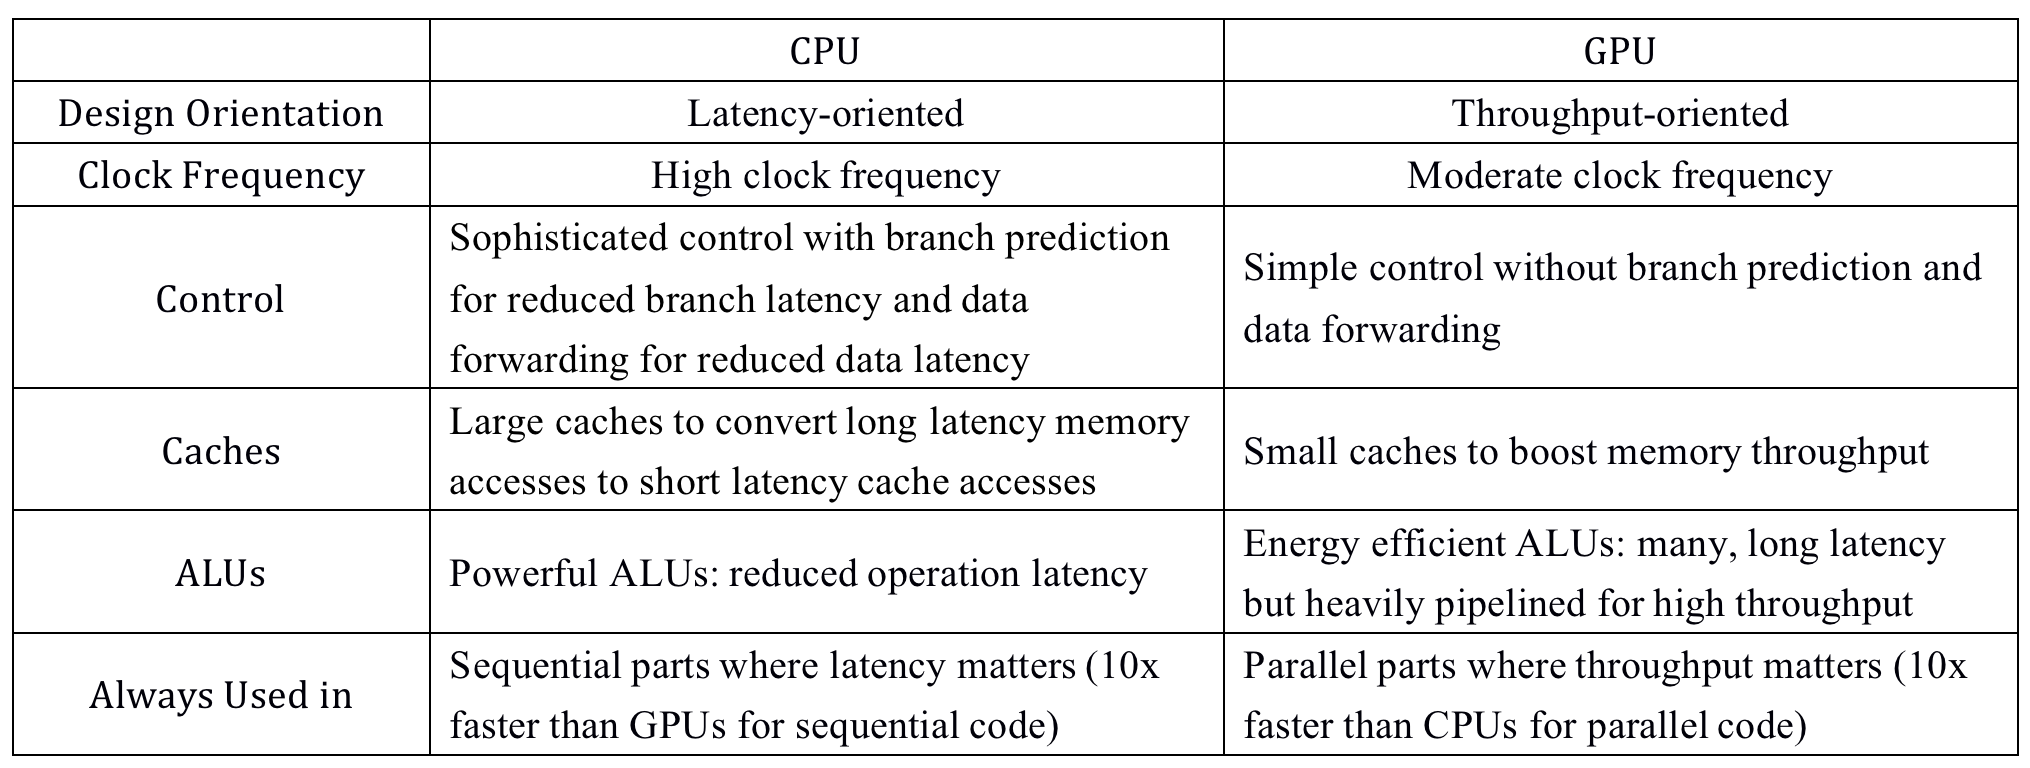
\includegraphics[width=15cm]{cpugpu.png}
\end{center}
\item(2-a) $12$ warps have control divergence, $20$ warps are inactive, $300$ threads are active, and $724$ threads are inactive.
\item \textbf{\textit{Proof}}: For the kernel with block dimension of $(64, 16)$, we need $64 \times 16 \times \frac{1}{32} = 32$ warps in total. Because each thread is able to process a subpart of the image of size $(16, 32)$, while the image is of size $(400, 384)$, $\frac{400}{16} = 25$, $\frac{384}{32} = 12$, so the threads active are of size $(25, 12)$, and totally $300$ threads are active, $724$ threads are inactive. Therefore, $12$ warps with blockIdx.y < $12$ (blockIdx.y starts with $0$) are active, and the rest $20$ warps are inactive.
\item (2-b) Let's have gridDim of $(1, 1, 1)$ and blockDim of $(16, 12, 1)$, and each thread is able to process a subpart of the image of size $(25, 32)$ ($25 \times 16 = 400, 12 \times 32 = 384$) such that there is no control divergence.
\begin{center}
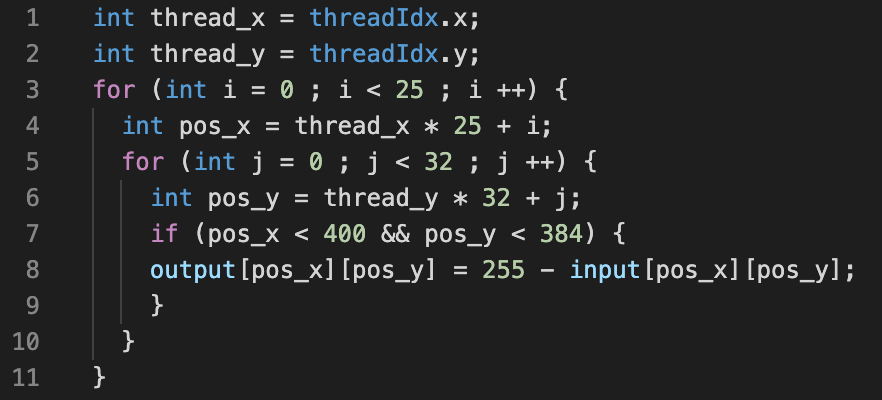
\includegraphics[width=10cm]{2.png}
\end{center}
\item (3) 
\begin{itemize}
\item For regular matrix multiplication of two $4$ by $4$ matrices: (1) We need to access the global memory for $16 \times 4 = 64$ times (because each thread needs to load elements from matrices for $4$ times), and $500$ cycles are needed to read from/write to the global memory, $1$ cycle is needed to read from/write to the registers, there are totally $64 \times 501 = 32,064$ cycles. (2) To write results back to the global memory, it takes $16 \times 500 = 8,000$ cycles. (3) So in general, $32,064 + 8,000 = 40,064$ cycles are needed.
\item For tiled matrix multiplication of two $4$ by $4$ matrices with TILE\_WIDTH = $2$. (1) We need to access the global memory and load data to the shared memory for $4 \times 2 = 8$ times (because each thread in a block deals with $2$ tiles, and $4$ blocks access data one by one), and $500$ cycles are needed to read from/write to the global memory, $5$ cycle is needed to read from/write to the shared memory, there are totally $8 \times 505 = 4,040$ cycles. (2) We need to access the shared memory to load data for $4 \times 6 = 24$ cycles. (3) To write results back to the global memory, it takes $4 \times 500 = 2,000$ cycles. (4) So in general, $4,040 + 24 + 2,000 = 6,064$ cycles are needed.
\end{itemize}
\item (4) The answer is $5$.
\item The number of parallel instructions is $5,120,000 \times 0.75 = 3,840,000$, and the number of sequential instructions is $1,280,000$, so for CPU + GPU computation, CPU needs $12,800,000$ cycles, and GPU needs $3,840,000 \times 250 \times 0.75 \times \frac{1}{1024n} = \frac{937,500}{n}$ cycles.
\item Compared to pure CPU computation, the relationship is:
\item $3.94225 = \frac{51,200,000}{12,800,000 + \frac{937,500}{n}}$
\item And we can find that $n \approx 5$.
\end{solution}
% ---------------------------------------------------------
\HomeworkHeader{2}{5}	% homework number, problem number
\setcounter{page}{10}
\begin{solution}
(A) By Amdahl’s Law,
\begin{center}
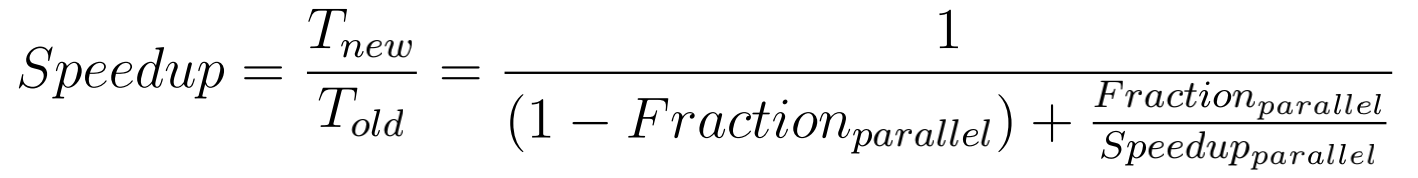
\includegraphics[width=12cm]{3.png}
\end{center}
If we want to speed up the application by a factor of $10$X, then we have the equation showing the fraction (percentage) of the code to be  parallelizable:
\item $Fraction_{parallel} = \frac{(10X-1) \cdot Speedup_{parallel}}{10X(Speedup_{parallel}-1)}$
\item (B-1) For total latency, 
\begin{center}
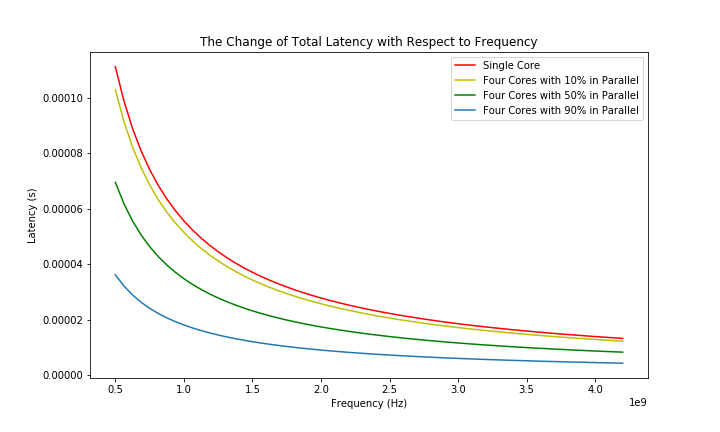
\includegraphics[width=15cm]{B1_1.png}
\end{center}
\pagebreak
For peak power,
\begin{center}
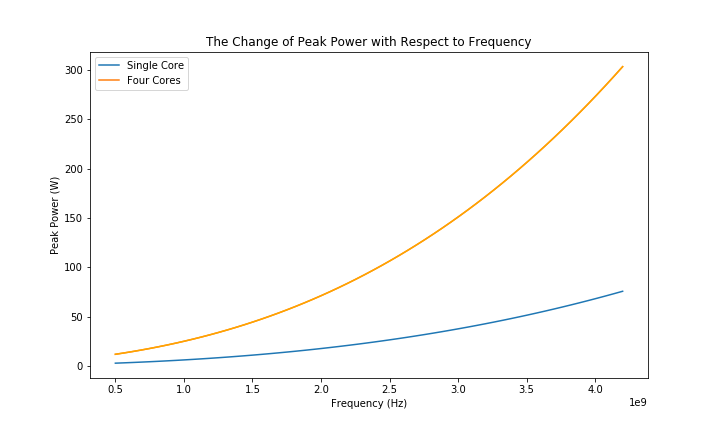
\includegraphics[width=15cm]{B1_2.png}
\end{center}
\item Notice that for four cores with $10\%, 50\%$, and $90\%$ in parallel, they have the same peak power.
\item For performance/average power,
\begin{center}
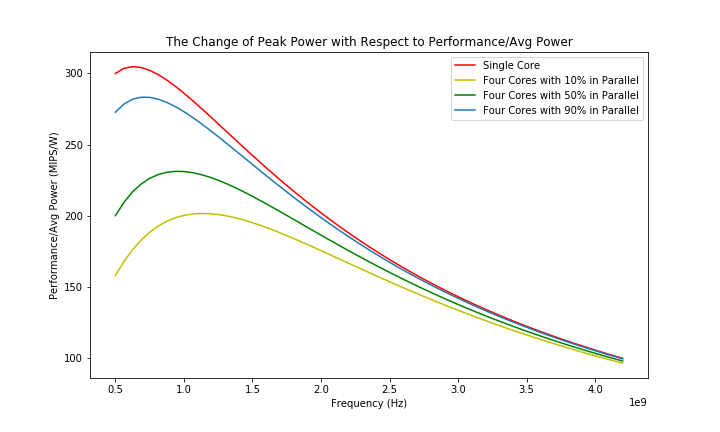
\includegraphics[width=15cm]{B1_3.png}
\end{center}
\pagebreak
\item (B-2)
\begin{center}
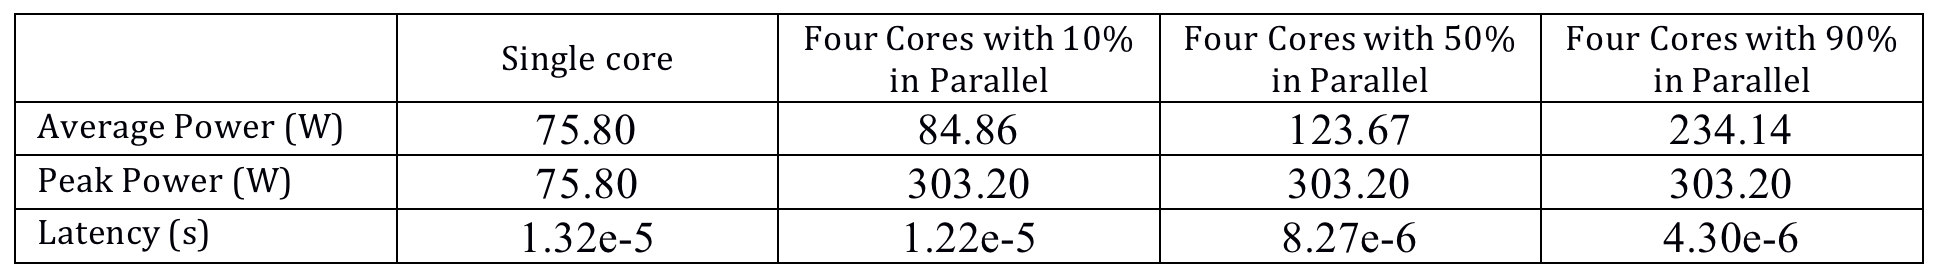
\includegraphics[width=15cm]{table.png}
\end{center}
\item (B-3) Performance per Watt is measured by performance/average power,
\begin{center}
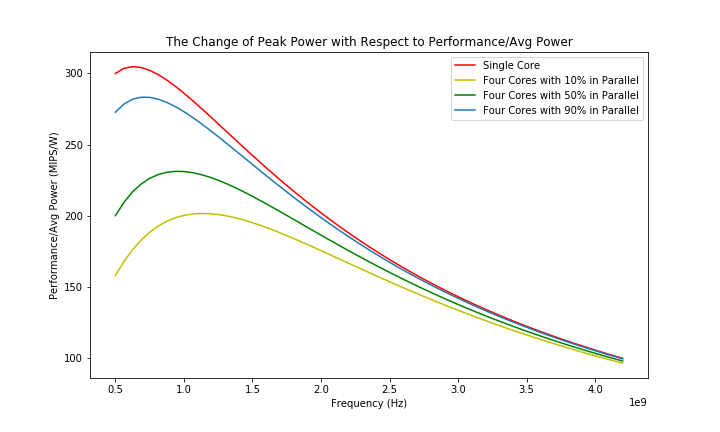
\includegraphics[width=15cm]{B1_3.png}
\end{center}
\item From the above plot, we could see at a frequency above $3.5$ GHz, the multi-core can achieve similar performance per Watt as the single-core.
\item If the static power per core is $2$W, the multi-core will be less energy-efficient, in order to achieve similar performance per Watt as the single-core, the multi-core should run at a higher frequency than the frequency when static power per core is $1$W.
\pagebreak
\item (B-4) The peak power changes as follows,
\begin{center}
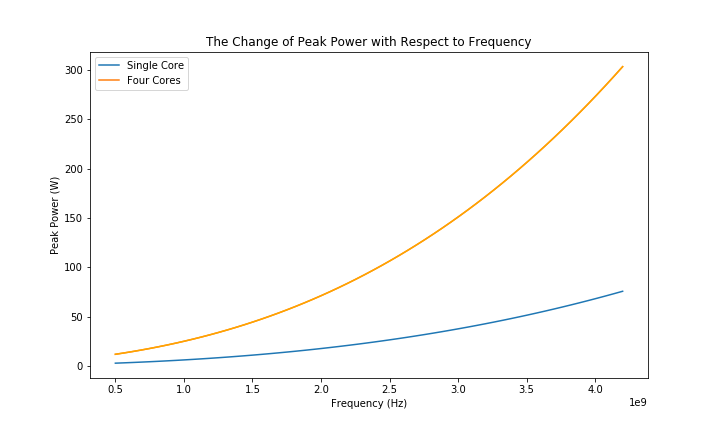
\includegraphics[width=15cm]{B1_2.png}
\end{center}
\item For the multi-core, parallelism will not influence peak power, so $10\%, 50\%, 90\%$ are all OK. For shorter latency and higher performance/average power, we should choose $90\%$, and remember to run the multi-core at a frequency below $1.5$ GHz.
\item (B-5) I will choose the four-core for $90$\% parallelism, and the two-core for $10$\% parallelism. Because when parallelism is high, we can exploit the advantage of more cores to reduce latency by choosing the four-core; but when parallelism is low, compared with high power consumption, the advantage of more cores is offset by low energy-efficiency.
\end{solution}
% ---------------------------------------------------------

\end{document}
